\documentclass[a4paper,10pt]{article}

%Math
\usepackage{amsmath}
\usepackage{amsfonts}
\usepackage{amssymb}
\usepackage{amsthm}
\usepackage{ulem}
\usepackage{stmaryrd} %f\"ur Blitz!
\usepackage{longtable} %fuer ASCII-Tabelle

%PageStyle
%\usepackage[utf8x]{inputenc}
\usepackage[german]{babel}
\usepackage{fontenc}
\usepackage{fancyhdr, graphicx}
\usepackage{wasysym}
\usepackage{fullpage}
\usepackage{textcomp}
\usepackage{fancyhdr} %for header/footer

%Zeichnung
\usepackage{tikz}
\usepackage[all]{xy}

\usepackage{color}
\usepackage{xcolor}
\usepackage{listings}

\usepackage{caption}
\DeclareCaptionFont{white}{\color{white}}
\DeclareCaptionFormat{listing}{\colorbox{gray}{\parbox{\textwidth}{#1#2#3}}}
\captionsetup[lstlisting]{format=listing,labelfont=white,textfont=white}

%lstlisting for java
\usepackage{listings}
  \usepackage{courier}
 \lstset{
         basicstyle=\footnotesize\ttfamily, % Standardschrift
         %numbers=left,               % Ort der Zeilennummern
         numberstyle=\tiny,          % Stil der Zeilennummern
         %stepnumber=2,               % Abstand zwischen den Zeilennummern
         numbersep=5pt,              % Abstand der Nummern zum Text
         tabsize=2,                  % Groesse von Tabs
         extendedchars=true,         %
         breaklines=true,            % Zeilen werden Umgebrochen
         keywordstyle=\color{red},
    		frame=b,         
 %        keywordstyle=[1]\textbf,    % Stil der Keywords
 %        keywordstyle=[2]\textbf,    %
 %        keywordstyle=[3]\textbf,    %
 %        keywordstyle=[4]\textbf,   \sqrt{\sqrt{}} %
         stringstyle=\color{white}\ttfamily, % Farbe der String
         showspaces=false,           % Leerzeichen anzeigen ?
         showtabs=false,             % Tabs anzeigen ?
         xleftmargin=17pt,
         framexleftmargin=17pt,
         framexrightmargin=5pt,
         framexbottommargin=4pt,
         %backgroundcolor=\color{lightgray},
         showstringspaces=false      % Leerzeichen in Strings anzeigen ?        
 }
 \lstloadlanguages{% Check Dokumentation for further languages ...
         %[Visual]Basic
         %Pascal
         %C
         %C++
         %XML
         %HTML
         Java
 }

%My Commands
\newcommand{\BN}{\mathfrak{B}} %Belegung
\newcommand{\RN}{\mathbb{R}} %Real Number
\newcommand{\NN}{\mathbb{N}} %Natural Number
\newcommand{\QN}{\mathbb{Q}} %Rational Number
\newcommand{\ZN}{\mathbb{Z}} %ganze Zahlen
\newcommand{\CN}{\mathbb{C}}
\newcommand{\Teilt}{\mid} %|
\newcommand{\Teiltn}{\nmid} %kein teiler
\newcommand{\Potp}{\mathcal{P}} %Potenzmenge
\newcommand{\Pota}{\mathcal{A}}
\newcommand{\Potr}{\mathcal{R}}
\newcommand{\Potn}{\mathcal{N}}
\newcommand{\Bold}[1]{\textbf{#1}} %Boldface
\newcommand{\Kursiv}[1]{\textit{#1}} %Italic
\newcommand{\T}[1]{\text{#1}} %Textmode
\newcommand{\Nicht}[1]{\T{\sout{$ #1 $}}} %Streicht Shit durch
\newcommand{\lra}{\leftrightarrow} %Arrows
\newcommand{\ra}{\rightarrow}
\newcommand{\la}{\leftarrow}
\newcommand{\lral}{\longleftrightarrow}
\newcommand{\ral}{\longrightarrow}
\newcommand{\lal}{\longleftarrow}
\newcommand{\Lra}{\Leftrightarrow}
\newcommand{\Ra}{\Rightarrow}
\newcommand{\La}{\Leftarrow}
\newcommand{\Lral}{\Longleftrightarrow}
\newcommand{\Ral}{\Longrightarrow}
\newcommand{\Lal}{\Longleftarrow}
\newcommand{\Vektor}[1]{\vec{#1}}
\newcommand{\Brace}[1]{\left( #1 \right)} %()
\newcommand{\Bracel}[1]{\left\lbrace #1 \right.} %(
\newcommand{\Bracer}[1]{\right. #1 \right\rbrace} %)
\newcommand{\Brack}[1]{\left\lbrace #1 \right\rbrace} %{}
\newcommand{\Brackl}[1]{\left\lbrace #1 \right.} %{
\newcommand{\Brackr}[1]{\right. #1 \right\rbrace} %}
\newcommand{\Result}[1]{\underline{\underline{#1}}} %Doppelt unterstrichen
\newcommand{\Abs}[1]{\left| #1 \right|} %Absolutbetrag
\newcommand{\Norm}[1]{\Abs{\Abs{ #1 }}} %Norm
\newcommand{\Arrays}[1]{\left(\begin{array}{c}#1\end{array}\right)} %Array mit einer Kolonne ()
\newcommand{\Array}[2]{\left(\begin{array}{#1}#2\end{array}\right)} %Array mit n Kolonnen ()
\newcommand{\Bracka}[2]{\left\lbrace\begin{array}{#1}#2\end{array}\right\rbrace} %Array mit {}
\newcommand{\Brackal}[2]{\left\lbrace\begin{array}{#1} #2 \end{array}\right.} %Array mit {
\newcommand{\Brackar}[2]{\left.\begin{array}{#1} #2 \end{array}\right\rbrace} %Array mit }
\newcommand{\Sumone}[2]{\sum_{#2=1}^{#1}} %Summe von 1
\newcommand{\Sumz}[2]{\sum_{#2=0}^{#1}} %Summe von 0
\newcommand{\Sum}[2]{\sum_{#1}^{#2}} %Allgemeine Summe
\newcommand{\Oneover}[1]{\frac{1}{#1}} %1 \"uber igendwas
\newcommand{\Tablewt}[3]{\begin{table\cdot }[h]\caption{#1} \begin{tabular}{#2}{#3}\end{tabular}\end{table\cdot }} %Table mit Titel
\newcommand{\Oben}[2]{\overset{#1}{#2}} %etwas \"uber etwas anderem
\newcommand{\Unten}[2]{\underset{#1}{#2}} %etwas unter etwas anderem
\newcommand{\Bildcap}[2]{\begin{figure}[htb]\centering\includegraphics[width=0.2\textwidth]{#1} \caption{#2}\end{figure}} %Bild mit beschriftung
\newcommand{\Bildjpeg}[1]{\includegraphics[width=0.2\textwidth]{#1.jpeg}} %Bilder jpeg!!
\newcommand{\Bildjpg}[1]{\includegraphics[width=0.2\textwidth]{#1.jpg}} %Bilder jpg!!

\usepackage{ucs}
\author{Fabio Oesch, Claude Martin, Jan F\"assler, Christian Glatthard, Fabian Stebler}
\title{Algorithmen \& Datenstrukturen 1}
\date{2. Semester (FS 2012)}
\fancyfoot[C]{If you use this documentation for a exam, you should offer a beer to the authors!}

%Config
\renewcommand{\headrulewidth}{0pt}
\setlength{\headheight}{15.2pt}
\pagestyle{plain}

\begin{document}
% Titelbild
\maketitle
\thispagestyle{fancy}

\newpage


% Inhaltsverzeichnis
\pagenumbering{Roman}
\tableofcontents	  	


\newpage
\setcounter{page}{1}
\pagenumbering{arabic}

\section{Information und Daten}
\subsection{Bin\"ares Zahlensystem}
low: 0 bis 0.8 V\\
high: 2.4 bis 5 V\\
\subsection{Bit und Byte}
\begin{itemize}
\item eine Bitfolge der L\"ange $n$ k\"onnen $2^n$ Zust\"ande hergestellt werden
\item Bits werden mit Indizes von 0 bis n-1 nummeriert.
\item LSB: Bit mit kleinstem Index
\item MSB: Bit mit h\"ochstem Index
\end{itemize}
\begin{tabular}{l l l }
	KiByte: $2^{10}$ Byte &
	MiByte: $2^{20}$ Byte &
	GiByte: $2^{30}$ Byte
\end{tabular}

\subsection{Zahlen in Java}
\subsubsection{Positive Zahlen}
$\sum {b_i * B^i}$ mit $i \in [0,n-1]$ und $b_i$ gleich der Ziffer bei $i$. \\\\
\begin{tabular}{|c|c|c|c|c|c|c|c|}
\multicolumn{1}{c}{MSB}&\multicolumn{6}{c}{}&\multicolumn{1}{c}{LSB}\\ \hline
1&0&1&0&0&1&1&1\\\hline
\multicolumn{1}{c}{$2^7$}&\multicolumn{1}{c}{$2^6$}&\multicolumn{1}{c}{$2^5$}&\multicolumn{1}{c}{$2^4$}&\multicolumn{1}{c}{$2^3$}&\multicolumn{1}{c}{$2^2$}&\multicolumn{1}{c}{$2^1$}&\multicolumn{1}{c}{$2^0$}\\
\end{tabular}\\
$1\cdot 2^7+0\cdot 2^6+1\cdot 2^5+0\cdot 2^4+0\cdot 2^3+1\cdot 2^2+1\cdot 2^1+1\cdot 2^0=167$
\subsubsection{Ganze Zahlen (2er - Komplement)}
$-b_{n-1}*B^{n-1}+\sum b_i*B^i$ mit $i \in [0,n-2]$ und  $b_i$ Ziffer bei $i$.\\\\
\begin{tabular}{|c|c|c|c|c|c|c|c|}
\multicolumn{1}{c}{MSB}&\multicolumn{6}{c}{}&\multicolumn{1}{c}{LSB}\\ \hline
1&0&1&0&0&1&1&1\\\hline
\multicolumn{1}{c}{$-2^7$}&\multicolumn{1}{c}{$2^6$}&\multicolumn{1}{c}{$2^5$}&\multicolumn{1}{c}{$2^4$}&\multicolumn{1}{c}{$2^3$}&\multicolumn{1}{c}{$2^2$}&\multicolumn{1}{c}{$2^1$}&\multicolumn{1}{c}{$2^0$}\\
\end{tabular}\\
$-1\cdot 2^7+0\cdot 2^6+1\cdot 2^5+0\cdot 2^4+0\cdot 2^3+1\cdot 2^2+1\cdot 2^1+1\cdot 2^0=-89$\\
\subsubsection{Zahlendarstellung mit beliebiger Basis}
\begin{itemize}
\item bin\"ar (2): Ganzzahlen, die mit \Bold{0b} beginnen
\item octal (8): Ganzzahlen, die mit \Bold{0} beginnen
\item dezimal (10): Ganzzahlen, die \Bold{nicht mit 0} beginnen
\item  hexadezimal (16): Ganzzahlen, die mit \Bold{0x} beginnen
\end{itemize}

\subsubsection{Modulo mit Int}
\begin{itemize}
\item  7 \% 3 = 2 Rest 1 
\item  -7 \% 3 = -2 Rest -1 
\item  -7 \% -3 = 2 Rest -1 
\item  7 \% -3 = -2 Rest 1 
\end{itemize}

\subsection{Datentypen in JAVA}
\begin{tabular}{l c c l l}
	Name & Byte & Bit & kleinste Zahl & gr\"osste Zahl \\
	\hline
	\Bold {byte} & 1 & 8 & -128 & 127 \\
	\Bold {short} & 2 & 16 &-32.768 & 32.767 \\
	\Bold {char} & 2 & 16 & $\backslash$u0000 (0) & 	$\backslash$uFFFF (65.535) \\
	\Bold {int} & 4 & 32 & -2.147.483.648 & 2.147.483.647 \\
	\Bold {long} & 8 & 64 & -9.223.372.036.854.775.808 & 9.223.372.036.854.775.807 \\
	\Bold {float} & 4 & 32 & $1,40 * 10^{-45}$ & $3,40282346638528860 * 10^{38}$ \\
	\Bold {double} & 8 & 64 & $4,94065645841246544*10^{-324}$ & $1,79769313486231570*10^{308}$  \\
\end{tabular}



\subsection{Gleitkommazahlen}
Exponentialdarstellung: $(-1)^V * (1+M)*2^E$ \\
IEEE 754 Float: $(-1)^V * (1+M) * 2^{E-127}$ \\
IEEE 754 Double: $(-1)^V * (1+M) * 2^{E-1023}$ \\
\begin{description}
	\item[V] - Vorzeichen (float 1Bit / double 1 Bit)
	\item[M] - normalisierte Mantisse $(0 \leq M \leq 1)$ (float: 23 Bits / double: 52 Bits)
	\item[E] - Exponent (float: Signed-8-Bit $-$ 127  / double: Signed-11-Bit $-$ 1023)
\end{description} 
\begin{tabular}{|c|l|l|}
	\hline
	V & Exponent & Mantrisse \\
	\hline
\end{tabular}

\subsubsection{Beispiele (IEEE 754 32bit Float)}
\begin{description}
	\item[2.5] $=1.25*2^1$
	\item[-0.75] $=\underbrace{1}_{\ominus}\underbrace{01111110}_{126 - 127} \underbrace{100000...}_{1+2^{-1}}=-1.5*2^{-1}$
	\item[0.1] $=\underbrace{0}_{\oplus}\underbrace{01111011}_{123 - 127} \underbrace{100\overline{1100}.........}_{1+2^{-1}+2^{-4}+2^{-5}...}=1.6*2^{-4} = 0.100000001490116119384765625$ 
	\item Umrechnen von $-1313.3125$ zu IEEE 32-bit float:
	\begin{enumerate}
		\item Ganzzahlteil $1313_{10}=10100100001_2.$
		\item Nachkommateil\\
		\begin{tabular}{lll}
			0.3125&$\times2=0.625$& \Bold{0}\\
			0.625&$\times 2=1.25$ &\Bold{1}\\
			0.25&$\times 2 = 0.5$ &\Bold{0}\\
			0.5&$\times 2=1.0$ &\Bold{1}\\
		\end{tabular}
		\item Ganzzahlteil$.$Nachkommateil=$1313.3125_{10}=10100100001.0101_2$
		\item Normen \begin{flushleft}
		Komma verschieben bis nur noch eine 1 vor dem Komma steht. Exponent entspricht der Anzahl verschobener Stellen. \linebreak Verschiebung des Kommas nach links: positiver Exponent.\linebreak Verschiebung des Kommas nach rechts: negativer Exponent. \end{flushleft} $10100100001.0101_2=1.01001000010101_2\times2^{10}$
		\item Mantisse ist $01001000010101$, Exponent ist $10 + 127 = 137 = 10001001_2$, Vorzeichen ist 1.
		\item -1313.3125 ist 
		\begin{tabular}{|c|l|l|}
			\hline
			1 & 10001001 & 01001000010101000000000 \\
			\hline
		\end{tabular}
	\end{enumerate} 
\end{description}

\subsubsection{Spezialf\"alle}
\begin{description}
	\item[E=00000000 M=0] $\Rightarrow 0$
	\item[E=11111111 M=0 V=+] $\Rightarrow +\infty$
	\item[E=11111111 M=0 V=$-$] $\Rightarrow -\infty$
	\item[E=11111111 M$\neq$0] $\Rightarrow NaN$
\end{description}

\subsubsection{Division mit Null}
\begin{itemize}
	\item float f = $\pm$0.0f/$\pm$0.0f = $NaN$
	\item float f = 7.6f/0.0f = -7.6f/-0.0f = $+\infty$
	\item float f = -3.9f/0.0f = 3.9f/-0.0f = $-\infty$
\end{itemize}

\newpage
\section{Operationen \& Ausdr\"ucke}

\subsection{Auswertungsreihenfolge}
\begin{itemize}
	\item einstellige und mehrstellige Operatoren
		\begin{itemize}
			\item[1.] Teilausdr\"ucke in Klammern
			\item[2.] Ausdr\"ucke mit un\"aren Operatoren (pro Operand von rechts nach links)
			\item[3.] Teilausdr\"ucke mit mehrstelligen Operatoren gem\"ass Priorit\"atstabelle
		\end{itemize}
	\item mehrstellige Operatoren gleicher Priorit\"at \\
		bei gleicher Priorit\"at entscheidet die Assoziativit\"at (von links nach rechts oder von rechts nach links)
	\item Bewertungsreihenfolge von Operanden \\
		die Operanden eines Operators werden strikt von links nach rechts ausgewertet
\end{itemize}
\begin{center}
\begin{tabular}{|c|l|l|c|}
\hline
\Bold{Priorit\"at}&\Bold{Operatoren}&\Bold{Bedeutung}&\Bold{Assoziativit\"at}\\\hline\hline
1&[]&Array-Index&links\\
&()&Methodenaufruf&links\\
&.&Komponentenzugriff&links\\
&++&Postinkrement&links\\
&$--$&Postdekrement&links\\\hline
2&++&Pr\"ainkrement&rechts\\
&$--$&Pr\"adekrement&rechts\\
&+ $-$&Vorzeichen (un\"ar)&rechts\\
&$\sim$&bitweises Komplement&rechts\\
&!&logischer Negationsoperator&rechts\\\hline
3&(type)&Typ-Umwandlungt&rechts\\
&new&Erzeugung&rechts\\\hline
4&* { }/ { }\%&Multiplikation, Division, Rest&links\\\hline
5&+ -&Addition, Subratktion&links\\
&+&Stringverkettung&links\\\hline
6&$<<$&Linksshift&links\\
&$>>$&Vorzeichenbehafteter Rechtsshift&links\\
&$>>>$&Vorzeichenloser Rechtsshift&links\\\hline
7&$<$ $<=$&Vergleich kleiner, kleiner gleich&links\\
&$>$ $>=$&Vergleich gr\"osser, gr\"osser gleich&links\\
&instanceof&Typen\"uberpr\"ufung eines Objektes&links\\\hline
8&==&Gleichheit&links\\
&!=&Ungleichheit&links\\\hline
9&\& &bitweises UND&links\\\hline
10&$^\wedge$&bitweises Exclusiv-ODER&links\\\hline
11&$\mid$&bitweises ODER&links\\\hline
12&\&\& { } \& &logisches UND&links\\\hline
13&$\mid\mid$ { } $\mid$&logisches ODER&links\\\hline
14&? :&Bedingungsoperator&rechts\\\hline
15&=&Wertzuweisung&rechts\\\hline
&*= { }/= { }\%=&kombinierter Zuweisungsoperator&rechts\\
&+= { }-= { }$<<$=&&\\
&$>>$= { } $>>>$=&&\\
&\&= { }$^\wedge$= { }$\mid$=&&\\\hline

\end{tabular}
\end{center}

\subsection{Bitoperatoren}
\begin{tabular}{|c|c|c|c|c|c|}
	\hline
	& & \Bold {AND} & \Bold {OR} & \Bold {Negation} & \Bold {XOR} \\
	\Bold {a} & \Bold {b} & \Bold {a \& b} & \Bold {a $|$ b} & \Bold {$\sim$a} & \Bold {a $\wedge$  b} \\
	\hline
	0 & 0 & 0 & 0 & 1 & 0 \\
	0 & 1 & 0 & 1 & 1 & 1 \\
	1 & 0 & 0 & 1 & 0 & 1 \\
	1 & 1 & 1 & 1 & 0 & 0 \\
	\hline
\end{tabular}

\subsection{Schiebeoperatoren}
\begin{itemize}
	\item \Bold {Rechtsschiebe-Operatoren}
		\begin{itemize}
			\item vorzeichenbehaftet: $a >> b$, \Bold{Bsp:}$-9_{10} = 11110111_2 >> 1 = 11111011_2 = -5_{10}$
			\item vorzeichenlos: $a >>> b$, \Bold{Bsp:}$-9_{10} =  11110111_2 >>> 1 = 01111011_2 = 123_{10}$ 
		\end{itemize}
	\item \Bold {Linksschiebe-Operator}
		\begin{itemize}
			\item kann Vorzeichen ver\"andern:  $a << b$
			\item $y=3<<2\Ra y=00001100_2=12$ (F\"ur jeden linksschiebeoperator wird $\cdot 2$ gerechnet.)
		\end{itemize}
\end{itemize}

\subsection{Logische Operatoren}
\begin{description}
	\item[logische Negation:] !A
	\item[logisches UND:] A \&\& B  / A \& B \\
				(Bei zwei \& Zeichen wird erst A \"uberpr\"uft und B nur, falls A wahr ist.)
	\item[logisches ODER:] A $||$ B / A $|$ B
	\item[Bedingungsoperator:] A ? B : C (if (A) then B else C)
\end{description}

\subsection{Beispiele}
\lstinputlisting[label=OneBitCounter,caption=OneBitCounter]{OneBitCounter.java}
\pagebreak
\lstinputlisting[label=Addition,caption=Addition]{Addition.java}
\lstinputlisting[label=Multiplication,caption=Multiplication]{Multiplication.java}

\newpage
\section{Konvertierung von Datentypen}

\subsubsection{explizite Typkonvertierung}
\begin{itemize}
	\item Konvertierungen sind m\"oglich:
		\begin{itemize}
			\item zwischen numerischen Datentypen (\Bold {erweiternd und einschr\"ankend})
			\item zwischen Referenztypen
		\end{itemize}
	\item funktionieren gleich wie implizite, allerdings bestehen mehr M\"oglichkeiten
	\item cast-Operator: (Typname) Ausdruck
\end{itemize}

\subsubsection{implizite (automatische) Typkonvertierung}
\begin{itemize}
	\item zwischen Operanden von numerischem Typ (\Bold {nur erweiternd})
	\item zwischen Operanden von Referenztypen
	\item bei Verkn\"upfungen von String-Objekten mit Operanden anderer Typen \\
			    Object o = new Object();\\
			    String s = $"$X$"$+null+o;\\
			   String s = $"$X$"$+$"$null$"$+o.toString();\\
                                   String s = $"$Xnulljava.lang.Object@47ac1adf$"$;
	\item arithmetische Operatoren: Konvertierung in h\"oheren Typ gem\"ass Hierarchie
\end{itemize}
\subsubsection{erweiternde Typkonvertierungen}
		Wert ist immer darstellbar \\
		m\"oglicher Verlust an Genauigkeit (z.B. bei Konvertierung von int nach float) \\ \\
		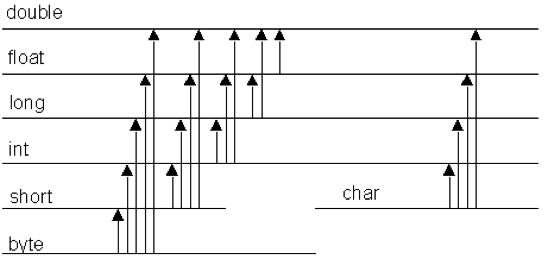
\includegraphics[width=75mm]{erweiternde_typumwandlung.png} \\
		
\subsubsection{einschr\"ankende Typkonvertierungen}
		m\"oglicher Informationsverlust in Gr\"osse, Vorzeichen \& Genauigkeit \\ \\
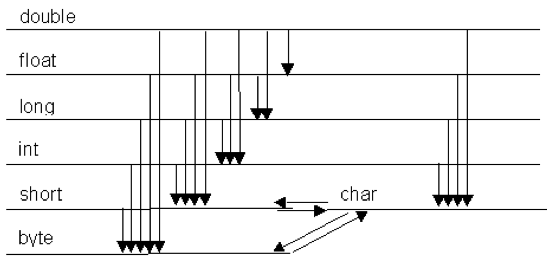
\includegraphics[width=75mm]{einschraenkende_typumwandlung.png}

\subsubsection{Integer-Erweiterung}
\begin{itemize}
	\item Datentypen byte, short und char werden in Ausdr\"ucken mit un\"aren und bin\"aren Operatoren implizit in int konvertiert
		\begin{itemize}
			\item Dimensionsausdruck bei der Erzeugung von Arrays
			\item Indexausdruck in Arrays
			\item Operand der un\"aren Operatoren $+$ und $ - $
			\item Operand des Invertierungsoperators f\"ur Bits $\sim$
			\item Operanden der Schiebeoperatoren $>>$, $>>>$ und $<<$
		\end{itemize}
	\item byte, short und char werden somit fast ausschliesslich als Datenfelder f\"ur Klassen benutzt
\end{itemize}
\subsubsection{Konvertierungsvorschriften}
\begin{itemize}
	\item erweiternde Konvertierung von vorzeichenbehafteten Integer-Typen \\
		Wert bleibt unver\"andert
	\item Konvertierung zwischen char und vorzeichenbehafteten Integer-Typen
		\begin{itemize}
			\item char ist vorzeichenlos
			\item short: Bitmuster bleibt erhalten, da gleiche Breite. Negativ wenn $b_{15} = 1$. 
			\item char zu int: von links mit Nullen auff\"ullen. Positiv.
			\item char zu byte: Bits 0 bis 7 werden \"ubernommen. Negativ wenn $b_7 = 1$.
		\end{itemize}
	\item Konvertierung von Integer nach Gleitpunkt \\
		n\"achst h\"oherer oder niedriger darstellbarer Wert
	\item Konvertierung von Gleitpunkt nach Integer
		\begin{itemize}
			\item Nachkommastellen werden abgeschnitten
			\item bei Werten gr\"osser als $2^{31} - 1$ ist das Resultat nicht korrekt ($= 2^{31} - 1$)
		\end{itemize}
	\item Konvertierung zwischen Gleitpunkt-Typen
		\begin{itemize}
			\item float nach double: Wert bleibt unver\"andert
			\item double nach float: Wert im zul\"assigen Wertebereich von float, dann n\"achst h\"oherer oder niedriger darstellbarer Wert
		\end{itemize}
\end{itemize}
\subsection{Beispiele}
\begin{tabular}{|l|l|}
\hline
\Bold{Umwandlung}&\Bold{Resultat}\\\hline\hline

(int) Double.MAX\_VALUE & Integer.MAX\_VALUE \\\hline
(int) (float) Integer.MAX\_VALUE & Integer.MAX\_VALUE \\\hline
(int) (float) (Integer.MAX\_VALUE - 1) & Integer.MAX\_VALUE (Genauigkeit ist nicht gegeben!)\\\hline
(int) Long.MAX\_VALUE & -1\\\hline
(int) Long.MIN\_VALUE & 0 \\\hline

(byte)(char) 254 & -2 \\\hline
(char)(byte) -2 & 65534 (falsch) \\\hline
(char)(byte) -2 $\&$ 0xff & 254 (korrekt) \\\hline
\hline
\end{tabular}



\pagebreak
\section{Zeichen und Strings}
\subsection{Zeichen in Java}
\begin{itemize}
\item int: 32-Bit im Format: nur die unteren 21 Bits werden benutzt, die oberen sind alle 0; eine int-Variable kann jeden m\"oglichen Zeichencode (code point) des Unicodes aufnehmen
\item char: 16 Bit; eine char-Variable kann nur einen der ersten $2^{16}$ Zeichencodes des Unicodes aufnehmen; alle anderen Zeichencodes werden durch char-Paare codiert (surrogate character mechanism)
\item Interface CharSequence: Sequenz von Zeichencodes im UTF-16 Format; bekannte Implementierung$\ra$ String, StringBuffer, StringBuilder, CharBuffer \ldots
\end{itemize}

\subsection{Standardisierte Zeichencodierungen}
\subsubsection{ASCII (American Standard Code for Information Interchange)}
\begin{itemize}
	\item nur 128 verschiedene Zeichen (Steuerzeichen, Satzzeichen, Ziffern, Buchstaben usw.)
	\item pro Zeichen ein eindeutiger 7-Bit-Zeichencode
\end{itemize}
\subsubsection{ISO 8859-1 (Latin-1)}
\begin{itemize}
	\item 256 Zeichen f\"ur europ\"aische Sprachen (8-Bit-Zeichencode)
	\item die ersten 128 Zeichen sind identisch zu ASCII
	\item die zweiten 128 Zeichen enthalten europ\"aische Sonderzeichen, z.B. Umlaute
\end{itemize}
\subsubsection{Unicode}
\begin{itemize}
	\item \"uber eine Million Zeichen, verschiedene Sprachen (Arabisch, Hebr\"aisch, Chinesisch usw.)
	\item 21-Bit-Zeichencode: ersten 256 Zeichen sind identisch zu ISO 8859-1
\end{itemize}

\subsection{Universal Character Encoding Standard (Unicode)}
\begin{description}
	\item[Ebene 0: Basic Multilingual Plane (BMP)] \hfill
		\begin{itemize}
			\item U+0 bis U+FFFF
			\item enth\"alt die wichtigsten Zeichen von verschiedenen Sprachen
		\end{itemize}
	\item[Ebene 1: Supplementary Multilingual Plane (SMP)] \hfill
		\begin{itemize}
			\item U+1'0000 bis U+1'FFFF
			\item enth\"alt weniger oft gebrauchte Zeichen (z.B. gotische Zeichen, Musiksymbole)
		\end{itemize}
	\item[Ebene 2: Supplementary Ideographic Plane (SIP)] \hfill
		\begin{itemize}
			\item U+2'0000 bis U+2'FFFF
			\item enth\"alt sehr seltene CJK Zeichen
		\end{itemize}
	\item[Ebene 3 bis 13] \hfill \\
		reserviert f\"ur sp\"atere Erg\"anzungen
	\item[Ebene 14: Supplementary Special-purpose Plane (SSP)] \hfill
		\begin{itemize}
			\item U+E'0000 bis U+E'FFFF
			\item enth\"alt zus\"atzliche Formatierungszeichen
		\end{itemize}
	\item[Ebenen 15 und 16: Private Use Planes] \hfill
		\begin{itemize}
			\item U+F'0000 bis U+F'FFFF und U+10'0000 bis 10'FFFF
			\item f\"ur private, nicht standardisierte Zwecke einsetzbar
		\end{itemize}
\end{description}

\subsubsection{UTF-32}
\begin{itemize}
\item einfachste Umsetzung: die 21 Bits werden in einem (vorzeichnlosen) 32-Bit-Integer abgespeichert; die h\"oherwertigen 11 Bits sind immer null
\item Vorteile: einfache Umsetzung; einheitliche Codierungsl\"ange
\item Nachteil: hohe Speicherverschwendung
\item Bsp: \\ A: U+0041 $\to$ 0000'0041 \\ $\Omega$: U+03A9 $\to$ 0000'03A9
\end{itemize}

\subsubsection{UTF-16}
\begin{itemize}
\item Umsetzung: Zeichencodes der BMP werden durch eine einzelne 16-Bit Codierungseinheit gespeichert; Zeichencodes der zus\"atzlichen Ebenen werden durch zwei 16-Bit Codierungseinheiten gespeichert $\to$ Ersatzpaare; guter Kompromiss zwischen Speicherbedarf und einfacher Handhabung
\item Ersatzpaare: beide Zeichen eines Ersatzpaares stammen aus der Surrogates Area; das erste Zeichen jeweils aus dem Bereich U+D800 bis U+DBFF; das zweite Zeichen jeweils aus dem Bereich U+DC00 und U+DFFF
\item Bsp: U+1'0384 $\to$ D800, DF84
    \begin{itemize}
    \item[1.] BMP abziehen: U+10384 - U+10000 = U+0384
    \item[2.] Umwandlung in bin\"ar und Aufteilung in 2*10 Bit Nutzdaten: \\
    0b$\underbrace{0000'0000'00}_{1. Zeichen} \underbrace{11'1000'0100}_{2. Zeichen}$
    \item[3.] Surrogate-Pr\"afixe hinzuf\"ugen\\
        \begin{itemize}
        \item 1. Zeichen: $\underbrace{1101'10}_{Praefix 1. Zeichen} \underbrace{0000'0000'00}_{1. Zeichen} $ = D800
        \item 2. Zeichen: $\underbrace{1101'11}_{Praefix 2. Zeichen} \underbrace{11'1000'0100}_{2. Zeichen} $ = DF84
        \end{itemize}
    \end{itemize}

\end{itemize}



\subsubsection{UTF-8}
\begin{itemize}
\item Bekannte Umsetzung: popul\"are Verwendung in XML; Zeichencodes brauchen zwischen 1 und 4 Bytes
\item Vorteile: speichereffizient f\"ur h\"aufig verwendete Zeichen; kompatibel mit ASCII
\item Nachteile: speicherineffizient f\"ur seltene Zeichen, jedoch nicht schlimmer als UTF-32; komplizierte Handhabung, weil unterschiedliche Anzahl von Bytes pro Zeichen beachtet werden muss; nicht kompatibel mit ISO-Latin-1, d.h. Umlaute brauchen bereits 2 Bytes
\item Bsp: \\ A: U+0041 $\to$ 41; \\ 
$\Omega$: U+03A9 $\to$ CE, A9; \\ 
Ugaritic Delta: U+10384 $\to$ F0, 90, 8E, 84
\end{itemize}
\begin{tabular}{|l|l|l|l|l|}
\hline
Zeichencode&Byte 1&Byte 2&Byte 3&Byte 4\\&&&&\\\hline
0xxxxxxx&\textcolor{red}{0}xxxxxxx&&&\\
&$\to$\textcolor{red}{1} byte&&&\\
&$\to$\textcolor{red}{7} bit (ASCII)&&&\\\hline
00000yyy&\textcolor{red}{110}yyyyy&\textcolor{green}{10}xxxxxx&&\\
yyxxxxxx&$\to$\textcolor{red}{2} byte&&&\\
&$\to$\textcolor{red}{11} bit&&&\\\hline
zzzzyyyy&\textcolor{red}{1110}zzzz&\textcolor{green}{10}yyyyyy&\textcolor{green}{10}xxxxxx&\\
yyxxxxxx&$\to$\textcolor{red}{3} byte&&&\\
&$\to$\textcolor{red}{16}bit (BMP)&&&\\\hline
000uuuzz&\textcolor{red}{11110}uuu&\textcolor{green}{10}zzzzzz&\textcolor{green}{10}yyyyyy&\textcolor{green}{10}xxxxxx\\
zzzzyyyy&$\to$\textcolor{red}{4} byte&&&\\
yyxxxxxx&$\to$\textcolor{red}{21}bit (alle)&&&\\\hline
\end{tabular}

\subsubsection{Codierungsschemen}
Das bestimmt Codierungsformat und Byte-Reihenfolge:
\begin{itemize}
	\item bei Dateneinheiten bestehend aus mehreren Bytes muss festgehalten werden, welches Byte zuerst behandelt wird, das
		\begin{itemize}
			\item most significant byte (MSB) zuerst: big-endian
			\item least significant byte (LSB) zuerst: little-endian
 		\end{itemize}		 
 	\item relevant bei UTF-16 und UTF-32
 	\item nicht relevant bei UTF-8 (die Reihenfolge ist klar)
 	\item durch Verwendung des Spezialzeichens Byte Order Mark (BOM) kann die Byte-Reihenfolge automatisch detektiert werden:
\end{itemize}

\subsection{Java}
\subsubsection{Unicode in JAVA}
\begin{description}
	\item[Datentyp int] \hfill 
		\begin{itemize}
			\item 32-Bit im UTF-32 Format: nur die unteren 21 Bits werden benutzt, die oberen sind alle 0
			\item eine int-Variable kann jeden m\"oglichen Zeichencode (code point) des Unicodes aufnehmen
		\end{itemize}
	\item[Datentyp char] \hfill 
		\begin{itemize}
			\item 16-Bit (Codierungseinheit, code unit)
			\item eine char-Variable kann nur einen der ersten $2^{16}$ Zeichencodes des Unicodes (Basic Multilingual Plane, BMP) aufnehmen
			\item alle anderen Zeichencodes werden durch char-Paare codiert
		\end{itemize}
	\item[Interface CharSequence] \hfill 
		\begin{itemize}
			\item Sequenz von Zeichencodes im UTF-16 Format
			\item bekannte Implementierungen: String, StringBuffer, StringBuilder
		\end{itemize}
\end{description}

\subsubsection{Zeichenketten (Strings)}
\begin{description}
	\item[Character-Array] \hfill \\
		ver\"anderbare Zeichenkette mit expliziter L\"angenangabe (Teil des Arrays)
	\item[Klasse String (UTF-16 Format)] \hfill \\
		unver\"anderbare Zeichenkette mit expliziter L\"angenangabe
	\item[Klassen StringBuilder und StringBuffer (UTF-16 Format)] \hfill \\
		ver\"anderbare Zeichenkette gekapselt als abstrakter Datentyp
\end{description}

\subsubsection{String Funktionen}
\begin{description}
	\item[String equals(String vergleichenMit)] \hfill \\
		vergleicht den Inhalt von zwei Strings
	\item[String substring(int anfang, int ende)] \hfill \\
		Schneidet eine Zeichenkette zwischen Anfang und Ende –1 aus und erzeugt damit ein neues Stringobjekt. Der urspr\"ungliche String wird dabei nicht ver\"andert.
	\item[String trim()] \hfill \\
		Erzeugt Kopie und entfernt alle Leerzeichen am Anfang und Ende der Kopie. Die Kopie wird zur\"uckgegeben.
\end{description}

\subsubsection{Umwandlungen}
\lstinputlisting[label=UTF 16 zu Latin1,caption=UTF 16 zu Latin1]{utfToLatin1.java}
\lstinputlisting[label=UTF 32 zu UTF 16,caption=UTF 32 zu UTF 16]{utf32to16.java}

\newpage
\subsection{ASCII-Zeichentabelle}
{\footnotesize
\begin{longtable}{|c|c|c|c||c|c|c|c|}
\hline
Dez & Hex & Okt & Zeichen & Dez & Hex & Okt & Zeichen\\
\hline
0 & 0x00 & 000 & NUL & 32 & 0x20 & 040 & SP\\
1 & 0x01 & 001 & SOH & 33 & 0x21 & 041 & ! \\
2 & 0x02 & 002 & STX & 34 & 0x22 & 042 & "'\\
3 & 0x03 & 003 & ETX & 35 & 0x23 & 043 & \# \\
4 & 0x04 & 004 & EOT & 36 & 0x24 & 044 & \$ \\
5 & 0x05 & 005 & ENQ & 37 & 0x25 & 045 & \% \\
6 & 0x06 & 006 & ACK & 38 & 0x26 & 046 & \& \\
7 & 0x07 & 007 & BEL & 39 & 0x27 & 047 & ' \\
8 & 0x08 & 010 & BS & 40 & 0x28 & 050 & (  \\
9 & 0x09 & 011 & TAB & 41 & 0x29 & 051 &  ) \\
10 & 0x0A & 012 & LF & 42 & 0x2A & 052 & * \\
11 & 0x0B & 013 & VT & 43 & 0x2B & 053 & + \\
12 & 0x0C & 014 & FF & 44 & 0x2C & 054 & , \\
13 & 0x0D & 015 & CR & 45 & 0x2D & 055 & $-$ \\
14 & 0x0E & 016 & SO & 46 & 0x2E & 056 & . \\
15 & 0x0F & 017 & SI & 47 & 0x2F & 057 & / \\
16 & 0x10 & 020 & DLE & 48 & 0x30 & 060 & 0 \\
17 & 0x11 & 021 & DC1 & 49 & 0x31 & 061 & 1 \\
18 & 0x12 & 022 & DC2 & 50 & 0x32 & 062 & 2 \\
19 & 0x13 & 023 & DC3 & 51 & 0x33 & 063 & 3 \\
20 & 0x14 & 024 & DC4 & 52 & 0x34 & 064 & 4 \\
21 & 0x15 & 025 & NAK & 53 & 0x35 & 065 & 5 \\
22 & 0x16 & 026 & SYN & 54 & 0x36 & 066 & 6 \\
23 & 0x17 & 027 & ETB & 55 & 0x37 & 067 & 7 \\
24 & 0x18 & 030 & CAN & 56 & 0x38 & 070 & 8 \\
25 & 0x19 & 031 & EM & 57 & 0x39 & 071 & 9 \\
26 & 0x1A & 032 & SUB & 58 & 0x3A & 072 & : \\
27 & 0x1B & 033 & ESC & 59 & 0x3B & 073 & ; \\
28 & 0x1C & 034 & FS & 60 & 0x3C & 074 & $<$ \\
29 & 0x1D & 035 & GS & 61 & 0x3D & 075 & =\\
30 & 0x1E & 036 & RS & 62 & 0x3E & 076 & $>$ \\
31 & 0x1F & 037 & US & 63 & 0x3F & 077 & ? \\
\hline

Dez & Hex & Okt & Zeichen & Dez & Hex & Okt & Zeichen\\
\hline
64 & 0x40 & 100 & @ & 96 & 0x60 & 140 & ` \\
65 & 0x41 & 101 & A & 97 & 0x61 & 141 & a \\
66 & 0x42 & 102 & B & 98 & 0x62 & 142 & b \\
67 & 0x43 & 103 & C & 99 & 0x63 & 143 & c \\
68 & 0x44 & 104 & D & 100 & 0x64 & 144 & d \\
69 & 0x45 & 105 & E & 101 & 0x65 & 145 & e \\
70 & 0x46 & 106 & F & 102 & 0x66 & 146 & f \\
71 & 0x47 & 107 & G & 103 & 0x67 & 147 & g \\
72 & 0x48 & 110 & H & 104 & 0x68 & 150 & h \\
73 & 0x49 & 111 & I & 105 & 0x69 & 151 & i \\
74 & 0x4A & 112 & J & 106 & 0x6A & 152 & j \\
75 & 0x4B & 113 & K & 107 & 0x6B & 153 & k \\
76 & 0x4C & 114 & L & 108 & 0x6C & 154 & l \\
77 & 0x4D & 115 & M & 109 & 0x6D & 155 & m \\
78 & 0x4E & 116 & N & 110 & 0x6E & 156 & n \\
79 & 0x4F & 117 & O & 111 & 0x6F & 157 & o \\
80 & 0x50 & 120 & P & 112 & 0x70 & 160 & p \\
81 & 0x51 & 121 & Q & 113 & 0x71 & 161 & q \\
82 & 0x52 & 122 & R & 114 & 0x72 & 162 & r \\
83 & 0x53 & 123 & S & 115 & 0x73 & 163 & s \\
84 & 0x54 & 124 & T & 116 & 0x74 & 164 & t \\
85 & 0x55 & 125 & U & 117 & 0x75 & 165 & u \\
86 & 0x56 & 126 & V & 118 & 0x76 & 166 & v \\
87 & 0x57 & 127 & W & 119 & 0x77 & 167 & w \\
88 & 0x58 & 130 & X & 120 & 0x78 & 170 & x \\
89 & 0x59 & 131 & Y & 121 & 0x79 & 171 & y \\
90 & 0x5A & 132 & Z & 122 & 0x7A & 172 & z \\
91 & 0x5B & 133 & [ & 123 & 0x7B & 173 & \{ \\
92 & 0x5C & 134 & $\backslash$ & 124 & 0x7C & 174 & $\mid$\\
93 & 0x5D & 135 & ] & 125 & 0x7D & 175 & \} \\
94 & 0x5E & 136 & \^{} & 126 & 0x7E & 176 & $\sim$ \\
95 & 0x5F & 137 & \_ & 127 & 0x7F & 177 & DEL \\
\hline
\end{longtable}
}
\newpage
\section{Suchen}
\subsection{Zahlensuche}
Generell gilt hier: Ordnung reduziert den Suchaufwand!
\subsubsection{Lineare Suche}
\lstinputlisting[label=Lineare Suche,caption=Lineare Suche]{lineare_suche.java}
\subsubsection{Lineare Suche mit W\"{a}chter (Sentinel)}
\lstinputlisting[label=Lineare Suche mit Waechter,caption=Lineare Suche mit Waechter]{suche_waechter.java}
\subsubsection{Bin\"are Suche}
\lstinputlisting[label=Binaere Suche,caption=Binaere Suche]{binarySearch.java}

\subsubsection{Analyse}
\begin{tabular}{l | l | c | c | c }
	Typ & Laufzeit & n & 256 & $2^{20}$ \\
	\hline
	Lineare Suche & lineare Laufzeit & n & 256 & $2^{20}$ \\
	Bin\"are Suche & logarithmisch & $[log_{2}(n)]+1$ & 9 & 21
\end{tabular}

\subsection{Textsuche}
\subsubsection{Naive Textsuche}
\begin{tabular}{l c c c c c c c l}
	text: & a & e & e & i & e & i & n & (n Zeichen) \\
	pattern: & e & i & n & & & & & (m Zeichen) \\
	& \lightning & e & i & n \\
	& & \checkmark & \lightning \\
	& & & e & i & n \\
	& & & \checkmark & \checkmark & \lightning \\
	& & & & e & i & n \\
	& & & & \lightning & e & i & n \\
	& & & & & \checkmark & \checkmark & \checkmark \\
\end{tabular} \\ \\
Auswertung: $T(n,m) = m(n-m+1)=m*n-m^2+m$

\subsubsection{Knuth-Morris-Pratt (KMP)}
Als erstes wird beim KMP das zu suchende Pattern untersucht. Das Pattern wird mit sich selber verglichen. Das Ziel ist zu wissen, bei welchem Buchstaben des Patterns man bei einem Missmatch weitermachen soll. \\
Es wird f\"ur jedes Teilst\"uck des Patterns das Endst\"uck maximaler L\"ange gesucht, welches einem Anfangsst\"uck entspricht. Dann wird abgespeichert, wo mit dem Vergleichen fortgefahren werden muss, wenn an dieser Stelle ein Fehler auftritt. \\ \\
\begin{tabular}{|c|c|c|c|c|c|c|c|}
	\hline 
	0 & 1 & 2 & 3 & 4 & 5 & 6 & 7 \\
	\hline
	h & a & u & s & h & a & l & t \\
	\hline
	-1 & 0 & 0 & 0 & 0 & 1 & 2 & 0 \\
	\hline
\end{tabular} \\ \\ \\
\begin{tabular}{|c|c|c|c|c|c|c|c|c|c|c|c|c|c|c|c|c|c|c|c|c|c|c|c|}\hline 
	0 &  1 &  2 &  3 &  4 &  5 &  6 &  7 &  8 &  9 &  0 &  1 &  2 &  3 &  4 &  5 &  6 &  7 &  8 &  9 &  0 &  1 &  2 &  3 \\\hline
	P &  A &  R &  T &  I &  C &  I &  P &  A &  T &  E &  &  I &  N &   &  P &  A &  R &  A &  C &  H &  U &  T &  E  \\\hline
	-1 &  0 &  0 &  0 &  0 &  0 &  0 &  0 &  1 &  2 &  0 &  0 &  0 &  0 &  0 &  0 &  1 &  2 &  3 &  0 &  0 &  0 &  0 &  0 \\\hline
\end{tabular}
\\ \\ \\

Die Tabelle Zeigt die Verschiebeinformationen f\"ur das Beispiel. Wenn beim Vergleich der Position 5 mit dem Text ein Fehler auftritt, dann muss bei Position 1 (also 1 wieder verglichen werden). Nur f\"ur den Anfangsbuchstaben ist der Wert -1. Wenn dieser genommen wird, heisst das, dass das Pattern wieder von vorne verglichen werden muss. \\
Diese Verschiebeinformationen werden zu Beginn der Suche im Text berechnet. Damit muss bei der Suche nie ein Teilst\"uck zweimal durchsucht werden. \\

\pagebreak
\Bold{Implementierung:}
\lstinputlisting[label=Knuth-Morris-Pratt,caption=Knuth-Morris-Pratt]{kpm.java}

\pagebreak
\section{Sortieren}
Ein Array a ist sortiert, wenn gilt: \\
$ \forall i \in [0, a.lenght-2] : a[i]\ relop\ a[i+1]$ \\
relop: Relation, Bin\"ares Pr\"adikat (typisch: $\leq,\geq,<,>$)

\subsection{\"Uberpr\"ufen, ob das Array sortiert ist}
\lstinputlisting[label=Ist Array sortiert?,caption=Ist Array sortiert?]{array_sorted.java}
Aufwand: linear in der L\"ange des Arrays \\

\subsection{Sortieren durch direktes Ausw\"ahlen (selection sort)}
Das Array wird durch gegangen und nach dem gr\"ossten Element durchsucht. Einmal gefunden, wird es hinten hingesetzt. Danach wird das zweitgr\"osste Element gesucht und vor das gr\"osste Element gestellt. Wenn man dies weiterf\"uhrt w\"achst der sortierte Teil des Arrays kontinuierlich, w\"ahrend der unsortierte Teil kleiner wird.
\lstinputlisting[label=Selection Sort,caption=Selection Sort]{selection_sort.java}
Worst-Case Aufwand: $T(n)=1+2+3+...+(n-3)+(n-2)+(n-1)=\sum_{k=1}^{n-1} k=\frac{n(n-1)}{2}=\frac{n^2-n}{2}\approx\uuline{\frac{n^2}{2}}$

\subsection{Sortierten durch direktes einf\"ugen (insertion sort)}
Das Array wird durch gegangen und jedes Element an der richtigen Stelle, der bereits durch gegangenen Elemente, eingesetzt.
\lstinputlisting[label=Insertion Sort,caption=Insertion Sort]{insertion_sort.java}
Worst-Case Aufwand: $T(n)=1+2+3+...+(n-3)+(n-2)+(n-1)=\sum^{n-1}_{k=1} k=\frac{n(n-1)}{2}=\frac{n^2-n}{2}\approx\uuline{\frac{n^2}{2}}$
Durchschnitt: $T(n)=0.5 + 1 + 1.5 + ... + \frac{(n-3)}{2} + \frac{(n-2)}{2} + \frac{(n-1)}{2}  + \frac{n}{2}=\sum^{n-1}_{i=1} \frac{i}{2}=\frac{1}{2}*\sum^{n-1}_{i=1} i = \frac{1}{2}*(\frac{n^2-n}{2})\approx\uuline{\frac{n^2}{4}}$

\subsection{Enumeration Sort}
Durchlaufe das gegebene Array a und vermerke jedes Auftreten eines Wertes u in einem Hilfsarray t an der Position p, wobei p sehr einfach aus u berechnet werden kann; d.h. t[p] muss zu Beginn 0 sein und wird mit jedem Auftreten von u um eins erh\"ot. \\
Durchlaufe t und schreibe jeweils fortlaufend t[p] mal den wert u  in das Array a.
\lstinputlisting[label=Enumeration Sort,caption=Enumeration Sort]{enumeration_sort.java}
\subsection{Quicksort (randomisierter Algorightmus)}
\begin{itemize}
	\item[0.] falls A.length $<=$ 1: Array A ist schon sortiert
	\item[1.] w\"ahle zuf\"allig ein Pivotelement p aus A und teile A wie folgt auf:
		\begin{itemize}
			\item[$A_1$:] enth\"alt nur Elemente aus A $\backslash$ p, die $<= p$ sind
			\item[$A_2$:] enth\"alt nur Elementa us A $\backslash$ p, die $>= p$ sind 
		\end{itemize}
	\item[2.] quicksort($A_1$) \\
		quicksort($A_2$)
	\item[3.] $A = [A_1, p, A_2]$
\end{itemize}
\subsubsection{Implementierung}
\lstinputlisting[label=Quicksort,caption=Quicksort]{quicksort.java}
\subsubsection{Aufwand Quicksort}
\begin{description}
	\item[Worstcase: Es wird immer das Element ganz links (bzw. ganz rechts) genommen]
	\begin{align*}
		T(1) &= 0\\
		T(n) &= c_1 + c_2 * n + T(1) + T(n-1)  = c_1 + c_2 * n + 0 + T(n-1) \\
		&= c_1 + c_2 * n + (c_1 + c_2 * (n - 1) + T(n - 2))\\ 
		&= 2 * c_1 + c_2 * ((n-2) + (n-1) + n) + T(n-3) \\
		&= 2 * c_1 + c_2 * ((n-1) + n) + (c_1 + c_2 * (n-2) + T(n-3))\\
		&= 3 * c_1 + c_2 * ( (n - 2) + (n - 1) + n) + T(n-3) \\
		&= i * c_1 + c_2 * \sum_{k=0}^{i-1} (n-k) + T(n-i)\\ 
		&= i * c_1 + c_2 * (n * \sum_{k=0}^{i-1} 1 - \sum_{k=0}^{i-1} k) + T(n-1)\\
		&\Ra \T{ sei nun }i=n-1\\
		&= c_1 * (n-1) + c_2 * (n * (n-1) - \frac{(n-2) * (n-1)}{2}) + T(1) \\
		&= c_1 * (n-1) + c_2 * (n^2-n-\frac{n^2}{2} + \frac{3*n}{2} -1) \\
		&= c_1 * (n-1) + c_{15}:362 * (\frac{n^2}{2} + \frac{n}{2} -1) \\
		T(n) &\in O(n^2)
	\end{align*}
	\item[Bestcase: Das Array nimmt immer das Element, dass in der Mitte des Arrays ist]
	\begin{align*}
		T(1) &= 0 \\
		T(n) &= c_1 + c_2 * n + 2 * T(\frac{n}{2}) \\
		&= 2 * T(\frac{n}{2}) + c_2 * n + c_1 \\
		&= 2 *(2 * T(\frac{n}{4})+c_2*\frac{n}{2} + c_1) + c_2 * n + c_1\\ 
		&= 4  * T(\frac{n}{4}) + c_4) + c_2 * n + 2 * c_1 + c_2 * n + c_1 \\
		&= 4 ( 2* T(\frac{n}{8}) + c_2 * \frac{n}{4} + c_1) + 2 * c_2*n+3*c_1\\
		&=8*T(\frac{n}{8}) + 3 *c_2 * n + 7* c_1\\
		&\Ra 2^i=n \T{ und } i=ld(n) \T{ werden ersetzt}\\
		&=2^i * T(\frac{n}{2^i}) + i * c_2 * n + \sum_{k=0}^{i-1} 2^k*c_1 \\
		&= n* T(\frac{n}{n}) +ld(n)*c_2*n+ c_1 * \sum_{k=0}^{ld(n)-1} 2^k \\
		&=c_2 * n * ld(n) + c_1 *(2^{ld(n)} -1) \\
		&=c_2 * n * ld(n) + c_1 * (n-1) \\
		&= n * (c_2 * ld(n) + c_1) - c_1  \\
		T(n) &\in O( n \cdot log~n)
	\end{align*}
\end{description}

\newpage
\subsection{Mergesort}
\lstinputlisting[label=Mergesort,caption=Mergesort]{mergesort.java}

\subsection{Laufzeiten}
\begin{tabular}{|l|l|l|l|l|}
\hline
Sortierverfahren&Best-Case&Average-Case&Worst-Case&Zus\"atzlicher Speicherplatz\\\hline\hline
Bubblesort&$O(n\cdot \log(n))$&$O(n\cdot \log(n))$&$O(n^2)$&\\\hline
Insertionsort&$O(n)$&$O(n^2)$&$O(n^2)$&\\\hline
Mergesort&$O(n\cdot \log(n))$&$O(n\cdot \log(n))$&$O(n\cdot \log(n))$&bei Array $O(n)$ bis $O(n\cdot \log(n))$\\\hline
Quicksort&$O(n\cdot \log(n))$&$O(n\cdot \log(n))$&$O(n^2)$&$O(n\cdot \log(n))$ f\"ur Stack\\\hline
Selectionsort&$O(n^2)$&$O(n^2)$&$O(n^2)$&\\\hline
\end{tabular}

\pagebreak
\section{Halbdynamische Datenstrukturen}
\subsection{Halbdynamische Datenstruktur}
\begin{description}
\item[statische Datestruktur]
	\begin{itemize}
		\item fixer Speicherbedarf, unabh\"angig von der Anzahl genutzter Elemente im Array
		\item direkter Zugriff auf die Elemente des Arrays
	\end{itemize}
\item[halbdynamische Datenstruktur]
	\begin{itemize}
	\item Speicherbedarf passt sich schrittweise der genutzten Anzahl Elemente an und bleibt zwischendrin konstant
	\item direkter Zugriff auf die Elemente
	\item Anpassung des Speicherbedarfs ist zeitaufw\"andig
	\end{itemize}
\item[dynamische Datenstrukturen (Liste, Stack, Baum usw.)]
	\begin{itemize}
	\item Speicherbedarf h\"angt direkt von der genutzten Anzahl Elemente ab
	\item \"ublich unterst\"utzte Operationen: Suchen, Einf\"ugen, Entfernen
	\item indirekter Zugriff auf die Elemente
	\end{itemize}
\end{description}
\subsection{Datennutzung \"uber die Zeit}
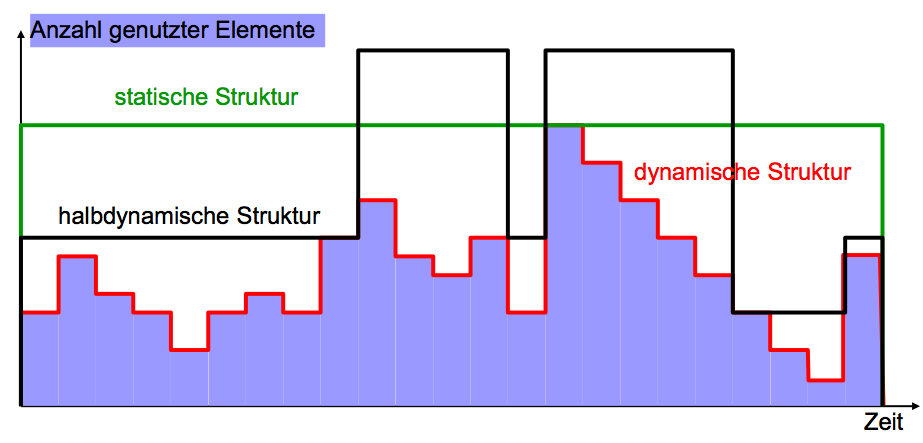
\includegraphics[width=1\textwidth]{datennutzung_ueber_zeit.png}
\subsection{Datenstruktur: ArrayList}
Implementiert das Interface list
\begin{itemize} \setlength{\itemsep}{-2pt}
	\item ArrayList verwendet intern ein Array von Objekten
	\item die L\"ange des Arrays entspricht der Kapazit\"at
	\item die verwendete Anzahl Elemente ist in size gespeichert
	\item Eine ArrayList startet mit der Gr\"osse 10 wenn nicht's anderes angegeben wurde
	\item Die Kapazit\"at wird erh\"oht, wenn die ArrayList voll ist und ein neues Element hinzugef\"ugt wird.
	\item Die neue Kapazit\"at wir bei der Erh\"ohung wie folgt berechnet:\\
			JRE1.6: $cap_{new}=(cap_{old} * 3) / 2 + 1$\\
			JRE1.7: $cap_{new}=cap_{old} + (cap_{old} >> 1)$
\end{itemize}

\begin{itemize}
	\item void add(int index, Object element)
	\item void clear()
	\item boolean contains(Object o)
	\item Object get(int index)
	\item int indexOf(Object o)
	\item boolean isEmpty()
	\item ListIterator listIterator(int index)
	\item Object remove(int index)
	\item boolean remove(Object o)
	\item Object set(int index, Object element)
	\item int size()
	\item \dots
\end{itemize}
\subsection{Generics Wildcards}
\subsubsection{Unbounded Wildcard $<$?$>$}
\begin{description}
\item[Einsatz]
	\begin{itemize}
	\item Deklaration einer Referenzvariable, die auf Objekte beliebiger aktuell parametrisierter Klassen eines generischen Typs zeigen kann
	\item Arrays von generischen Klassen
	\end{itemize}
\item[Interpretation]
	\begin{itemize}
	\item bei G$<$T$>$ steht der formale Typ-Parameter T stellvertretend f\"ur genau einene Referenztyp
	\item bei G$<$?$>$ steht das Fragezeichen f\"ur alle m\"oglichen Referenztypen
	\end{itemize}
\end{description}
\lstinputlisting[label=Unbound Wildcard,caption=Unbound Wildcard]{unbound_wildcard.java}

\subsubsection{Upper Bound Wildcard $<$? extends T$>$}
\begin{description}
\item[Einsatz] Deklaration einer Referenzvariable, die auf Objekte eines generischen Typs zeigen kann, wobei die Objekte mit T oder einer Subklasse von T aktuell parametrisiert sein m\"ussen
\item[Interpretation] bezeichnet die oberste Klasse in der Klassenhierarchie, welche als aktuellen Typ-Parameter f\"ur den formalen Typ-Parameter T eingesetzt werden darf
\end{description}
\lstinputlisting[label=Upper Bound Wildcard,caption=Upper Bound Wildcard]{upper_bound_wildcard.java}

\subsubsection{Low Bound Wildcard $<$? super T$>$}
\begin{description}
\item[Einsatz] Deklaration einer Referenzvariable, die auf Objekte eines generischen Typs zeigen kann, wobei die Objekte mti T oder einer Superklasse von T aktuell parametrisiert sein m\"ussen
\item[Interpretation] bei G$<$? super C$>$ steht das Fragezeichen f\"ur alle m\"oglichen Superklassen von C (inkl. C selber)
\end{description}
\lstinputlisting[label=Lower Bound Wildcard,caption=Lower Bound Wildcard]{lower_bound_wildcard.java}

\subsubsection{Interner Aufbau (bis Java 1.4.2)}
\begin{itemize}
	\item alle Klassen aus dem Java Collections Framework verwalten intern Referenzen vom Typ Object \\ $\Rightarrow$ maximale Flexibilit\"at
	\item alle Methodenschnittstellen verwenden den Typ Object
	\item da alle Referenztypen zur Klasse Object zuweisungskompatibel sind, bieten die Collections keine Typsicherheit
\end{itemize}

\subsubsection{Interner Aufbau (seit Java 5.0)}
\begin{itemize}
	\item alle Collections verwalten intern Referenzen vom Typ $<$E$>$, wobei E ein beliebiger Platzhalter (Typ-Parameter) f\"ur einen konkreten Referenztyp ist
	\item Collections werden generisch (maximale Flexibilit\"at)
	\item Collections k\"onnen f\"ur alle m\"oglichen Referenztypen verwendet werden, auch
f\"ur Object (= fr\"uherer interner Aufbau)
\end{itemize}

\pagebreak
\section{Programmverifikation}
\subsection{Korrektheit eines Algorithmus}
\begin{itemize}
\item Ein Algorithmus heisst korrekt, wenn er seiner Spezifikation gen\"ugt
\item \"uberpr\"ufung:
	\begin{itemize}
	\item Verifikation: Mittels logischer Herleitung
	\item Testen: Fehlerfreiheit kann nicht nachtgewiesen werden
	\end{itemize}
\end{itemize}
\subsection{Aussagenlogik}
\subsubsection{Syntax}
\begin{itemize}
\item atomare Formeln (Atome): A, B, C, ...
\item seien F und G zwei beliebige Formeln
\item Konjuktion: $(F\wedge G)$ ist eine Formel
\item Disjunktion: $(F\vee G)$ ist eine Formel
\item Negation: $neg F$ ist eine Formel
\item Implikation: $(F\to G)$ ist eine Kurzschreibweise f\"ur $(\neg F\vee G)$
\item Bikonditional: $(F\lra G)$ ist eine Kurzschreibweise f\"ur $(F\to G)\wedge(G\to F)$
\end{itemize}
\subsubsection{Semantik}
		\begin{itemize}
				\item Belegung $\mathfrak{B}$: eine Teilmenge der atomaren Formeln wird mit einem Wahrheitswert aus {false, true} bzw. {0,1} belegt
				\item die Bedeutungen der Konjunktion, Disjunktion und Negation sind analog zur Bool'schen Algebra definiert
				\item passende Belegung $\mathfrak{B}$ auf Formel F angewendet: $\mathfrak{B}$(F)
		\end{itemize}
		
\subsubsection{Modell}
		\begin{itemize}
			\item eine Belegung heisst zu einer Formel F \Bold {passend}, wenn alle in F
vorkommenden Atome belegt sind
			\item eine Belegung $\mathfrak{B}$ ist ein \Bold {Modell} f\"ur eine Formel F, wenn sie passend ist
und wenn der Wahrheitswert von $\mathfrak{B}$(F) = true ist: $\mathfrak{B} \models F$
			\item Belegung ist $\mathfrak{B}$ \Bold {kein Modell} f\"ur Formel F, wenn sie zwar passend ist,
aber wenn der Wahrheitswert von $\mathfrak{B}$(F) = false ist: $\mathfrak{B} \nvDash F$
		\end{itemize}
		
\subsubsection{Erf\"ullbarkeit}
\begin{itemize}
	\item Eine Formel F heisst \Bold {erf\"ullbar}, wenn f\"ur sie ein Modell existiert, andernfalls \Bold {unerf\"ullbar}
	\item Eine Formel F heisst \Bold {g\"ultig} (oder Tautologie), wenn alle passenden Belegungen Modelle sind: $ \models F$
\end{itemize}

\subsubsection{\"Aquivalenz}
Zwei Formeln F und G heissen (semantisch) \"aquivalent, falls f\"ur alle passenden Belegungen $\mathfrak{B}$ gilt:\\ $\mathfrak{B}$(F) = $\mathfrak{B}$(G). Daf\"ur schreiben wir $\models (F \leftrightarrow G)$ oder kurz $F \equiv G$. \\ 
\begin{tabular}{l l c | c l l}
\multicolumn{2}{c}{AND} &&& \multicolumn{2}{c}{OR} \\
\hline 
&&&&& \\
$(F \wedge F)$                    & $\equiv F$                                                 &&& $(F \vee F)$ & $\equiv F$ \\
$(F \wedge G)$                   & $\equiv (G \wedge F)$                               &&& $(F \vee G)$ & $\equiv (G \vee F)$ \\
$((F \wedge G) \wedge H)$ & $\equiv (F \wedge (G \wedge H))$             &&& $((F \vee G) \vee H)$ & $\equiv (F \vee (G \vee H))$ \\
$(F \wedge (F \vee G))$      & $\equiv F$                                                 &&& $(F \vee (F \wedge G))$ & $\equiv F$ \\
$(F \wedge (G \vee H))$     & $\equiv ((F \wedge G) \vee (F \wedge H))$ &&& $(F \vee (G \wedge H))$ & $\equiv ((F \vee G) \wedge (F \vee H))$ \\
$\neg (F \wedge G)$          & $\equiv (\neg F \vee \neg G)$                    &&& $\neg (F \vee G)$ & $\equiv (\neg F \wedge \neg G)$ \\
$(F \wedge G)$                  & $\equiv G$, falls $\models F$                    &&& $(F \vee G)$ & $ \equiv G$, falls $\models F$ \\
$(F \wedge G)$                  & $\equiv$ F, falls F unerf\"ullbar                 &&& $(F \vee G)$ & $\equiv$ F, falls F unerf\"ullbar \\

\end{tabular}

\subsection{Pr\"adikatenlogik}
\subsubsection{Syntax}
\begin{itemize}
	\item Erweiterung der Aussagenlogik um Quantoren, Funktionen, Pr\"adikate, Relationen und Variablen
		\begin{itemize} 
			\item nullstellige Pr\"adikate entsprechen den Atomen der Aussagelogik
			\item Relationen k\"onnen als Pr\"adikate aufgefasst werden
			\item nullstellige Funktionen sind Konstanten
		\end{itemize}
	\item Formeln
		\begin{itemize}
			\item logische Verkn\"upfung von Pr\"adikaten: \\
				die Argumente der Pr\"adikate sind Terme, gebildet aus Funktionen, Variablen und Konstanten
			\item sei x eine Variable und F eine Formel
				\begin{itemize}
					\item $\forall$ x F ist eine Formel mit gebundenem x
					\item $\exists$ x F ist eine Formel mit gebundenem x
				\end{itemize}
			\item eine Formel heisst geschlossen oder Aussage, wenn alle ihre Variablen durch Quantoren gebunden sind
		\end{itemize}
	\item Pr\"adikatenlogik mit Identit\"at \\
		wenn F und G zwei Formeln sind, so ist auch F = G eine Formel
\end{itemize}

\subsubsection{Semantik}
\begin{itemize}
	\item Struktur $S = (U_s, I_s)$ \\
		$U_s$ ist eine nicht-leere Grundmenge und $I_s$ eine Abbildung
		\begin{itemize}
			\item der Pr\"adikate \"uber $U_s$
			\item der Funktionen auf $U_s$
			\item der Variablen auf Elemente von $U_s$
		\end{itemize}
	\item Semantik bez\"uglich passender Struktur S
		\begin{itemize}
			\item[S(Term)] jeder Term wird gem\"ass $I_s$ auf ein Element aus $U_s$ abgebildet
			\item[S(Pr\"adikat)] jedes Pr\"adikat bestimmt einen Wahrheitswert in Abh\"angigkeit seiner Argumente (Terme)
			\item[S(Formel)] die aussagenlogische Verkn\"upfung der Wahrheitswerte der Pr\"adikate
			\item[S($\forall$x F)] F ist eine Formel 
				\begin{itemize}
					\item ist true, falls f\"ur alle d $\in$ $U_s$ gilt: $S_{[x/d]}(F) = true$
					\item ist false, sonst
				\end{itemize}
			\item[S($\exists$x F)] F ist eine Formel
				\begin{itemize}
					\item ist true, falls f\"ur alle d $\in$ $U_s$ gilt: $S_{[x/d]}(F) = true$
					\item ist false, sonst
				\end{itemize}
		\end{itemize}
\end{itemize}

\subsubsection{\"Aquivalenz}
\begin{description}
	\item[Definition] \hfill \\
		Zwei pr\"adikatenlogische Formeln F und G sind \"aquivalent, falls f\"ur alle passenden Strukturen S gilt: S(F) = S(G). Daf\"ur schreiben wir F $\equiv$ G.
	\item[\"Aquivalenzregeln (zus\"atzlich zur Aussagenlogik)] \hfill \\
	\begin{tabular}{rcl}
		$\neg \forall x F $&$\equiv$&$ \exists x \neg F$ \\
		$\forall x \forall y F $&$\equiv$&$ \forall y \forall x F$ \\
		$(\forall x F \wedge \forall x G) $&$\equiv$&$ \forall x (F \wedge G)$ \\
		$\neg \exists x F $&$\equiv$&$ \forall x \neg F$ \\		
		$\exists x \exists y F $&$\equiv$&$ \exists y \exists x F$ \\
		$(\exists x F \vee \exists x G) $&$\equiv$&$ \exists x (F \vee G)$ \\ \\
		falls x in G nicht frei vorkommt, gilt: \\
		$(\forall x F \wedge G) $&$\equiv$&$ \forall x (F \wedge G)$ \\
		$(\forall x F \vee G) $&$\equiv$&$ \forall x (F \vee G)$ \\
		$(\exists x F \wedge G) $&$\equiv$&$ \exists x (F \wedge G)$ \\
		$(\exists x F \vee G) $&$\equiv$&$ \exists x (F \vee G)$ \\
	\end{tabular}
\end{description}

\subsubsection{Beispiele}
\begin{description}
	\item[Alle Studierenden von Professor p m\"ogen Logik.] \hfill \\
		L(x) : "x mag Logik" \\
		S(x,y) : "x studiert bei y" \\
		$\forall x: S(x,p) \ra L(x)$ \\
		$\forall x: \neg S(x,p) \vee L(x)$
	\item[Ein Professor ist gl\"ucklich, wenn alle seine Studierenden Logik m\"ogen] \hfill \\
		G(x) : "x ist gl\"ucklich" \\
		$\exists y: (\forall x : S(x,y) \ra L(x)) \ra G(y)$
	\item[Ein Professor ist ungl\"ucklich, wenn er keine Studierende hat.] \hfill \\
		$\exists y: (\forall x : \neg S(x,y)) \ra \neg G(y))$
\end{description}

\subsection{Verifikation}
\subsubsection{Hoare-Tribble}
\Bold {Ein Hoare-Triple ( $\{ R \} P \{ S \}$ ) ist g\"ultig, wenn bei erf\"ullter Vorbedingung R und nach Ausf\"uhrung von P die Spezifikation (Nachbedingung) S erf\"ullt ist.} Das Programm P ist korrekt, wenn das Hoare-Triple g\"ultig ist.
\begin{description}
	\item[Variablen] \hfill \\
		Input: $a, b, c, ..., z$ \\
		Output: $a', b', c', ..., z'$
	\item[Vorbedingung (Precondition)] \hfill \\
		Damit das Programm P die Spezifikation (Postcondition) S erf\"ullen kann, muss die Vorbedingung R erf\"ullt sein. Je schw\"acher die Vorbedingung R, desto besser: \Bold {weakest precondition (WP)}.
	\item[Beispiele] \hfill \\
		Spezifikation: $S = (x' = 10)$ \\
		Programm: $P = (x' := x + 2)$ \\
		m\"ogliche Vorbedingung $R = (a = 0 \vee b = 2 \vee x = 8 \vee z = 0)$ \\
		einfachste Vorbedingung (weakest Precondition);  $WP = (x = 8)$
\pagebreak
	\item[Nachbedingungen (Postcondition)] \hfill \\
		Die Nachbedingungen entsprechen der \Bold {Spezifikation} des Programms und sind je pr\"aziser, umso besser. \\
		Implikation: $[\underbrace{S}_{spezielle Spez.} \ra \underbrace{T}_{allg. Spez.}] \equiv \forall a, b, c, ..., z, a', b', c', ..., z': \neg S \vee T$
		\begin{itemize}
			\item $a, b, c, ..., z$ sind alle Variablen, die in den Spezifikationen S und T vorkommen
			\item wenn ein Programm P die speziellere Spezifikation S erf\"ullt, so auch die allgemeinere T
			\item es gibt ein Programm Q, welches die Spezifikation T erf\"ullt und mindestens so einfach ist wie das Programm P, welches die Spezifikation S erf\"ullt
		\end{itemize}
	\item[Besipiele:] \hfill \\
		$S = (x' = 10), T = (x' > 0)$ \\
		$P_1 = (x' := 6), P_2 = (x' := 10), P_3 = (x' := x + 1)$
		\begin{itemize}
			\item $\underbrace{\{true\}}_{algemeinste Vorbedingung} P_1 \{S\} = false$
			\item $\{true\} P_1 \{T\} = true$
			\item $\{true\} P_2 \{S\} = true$
			\item $\{true\} P_2 \{T\} = true$
			\item $\{true\} P_3 \{S\} = false$
			\item $\{x=9\} P_3 \{S\} = true$
		\end{itemize}
\end{description}
\subsubsection{Ablauf der Verifikation}
\begin{description}
	\item[Gegeben] \hfill \\ \\
		Vorbedingung R, Spezifikation S, Programm P
	\item[Ablauf] \hfill 
		\begin{itemize}
			\item aus S und P die schw\"achste Vorbedingung $WP = wp(P, S)$ berechnen
			\item falls $[R \ra WP]$ gilt, dann erf\"ullt das Programm P die Spezifikation S bei eingehaltener Vorbedingung R
			\item R kann somit durch WP ersetzt werden
		\end{itemize}
	\item[Berechnung der WP] \hfill 
		\begin{itemize}
			\item ausgehend von der Spezifikation S
			\item Anweisung f\"ur Anweisung r\"uckw\"arts rechnen
			\item Berechnungsregeln f\"ur Zuweisung, Sequenz, Selektion, Iteration
		\end{itemize}
\end{description}

\subsection{Weakest Precondition: Rechenregeln}
\subsubsection{Zuweisung}
\begin{description}
	\item[Gegeben] \hfill \\
		Zuweisung $P = (x' := y)$ \\
		Nachbedingung S
	\item[Regel] \hfill \\
		$WP = wp(P, S) = wp((x' := y), S) = S |_{alle \hspace{2mm} x' \hspace{2mm} durch \hspace{2mm} y \hspace{2mm} ersetzt}$
	\item[Beispiele] \hfill \\
		$S = (a' = z), P = (a' := b + c), WP = (b + c = z)$ \\
		$S = (n' = n), P = (n' := n-1), WP = (n = n-1) = false$
\end{description}
\subsubsection{Weakest Precondition herausfinden (Beispiel)}
$S=(r'=x\cdot y)$, $P=(\T{if }x=2\cdot k ~then~ r' := 2\cdot k\cdot y\T{ else }s':=2\cdot k\cdot y;r':=s'+y)$, $B=(x=2\cdot k)$
\begin{align*}
S1&=wp((r':=2ky),S)=(2ky=xy)=(2k=x)=B\\
S2&=wp((s':=2ky;r':=s'+y),S)=wp(s':=2ky,s'+y=xy)=(2ky+y=xy)=(2k+1=x)\\
R&=wp(P,S)=(B\to S1\wedge\neg B\to S2)\\
&=(\neg B\vee S1)\wedge(B\vee S2)=\neg B\wedge B\vee\neg B\wedge S2\vee S1\wedge B\vee S1\wedge S2\\
&=\neg B\wedge S2\vee S1\wedge B \vee S1\wedge S2\\
&=B\wedge S1\vee\neg B\wedge S2\\
&=(x=2k\wedge x=2k)\vee(x\neq 2k\wedge 2k+1=x)\\
&=(x=2k)\vee(2k+1\neq 2k\wedge 2k+1=x)\\
&=(x=2k)\vee(true\wedge 2k+1=x)\\
&=(x=2k)\vee(x=2k+1)
\end{align*}
\subsubsection{Sequenz}
\begin{description}
	\item[Gegeben] \hfill \\
		Sequenz P = $(Anweisung_1; Anweisung_2; ...; Anweisung_n)$ \\
		Nachbedingung S
	\item[Regel] \hfill \\
		$WP = wp(P, S) =
wp((Anweisung_1; Anweisung_2; ...; Anweisung_{n-1}), wp(Anweisung_n, S))$
	\item[Beispiel] \hfill \\
		$P = (t' := x; x' := y; y' := t')$ \\
		$S = (x' = b \wedge y' = a)$ \\
		\begin{tabular}{ll}
		$WP $&$=wp((t':=x;x':=y;y':=t'),(x'=b \wedge y'=a))$ \\
		&$= wp((t' := x; x' := y), wp((y' := t'), (x' = b \wedge y' = a)))$ \\
		&$= wp((t' := x; x' := y), (x' = b \wedge t' = a))$ \\
		&$= wp((t' := x), wp((x' := y), (x' = b \wedge t' = a)))$ \\
		&$= wp((t' := x), (y = b \wedge t' = a))$ \\
		&$= (y = b \wedge x = a)$
		\end{tabular}
\end{description}

\subsubsection{Selektion}
\begin{description}
	\item[Gegeben] \hfill \\
		logischer Ausdruck b ;
		Selektion P = (if b then $P_1$ else $P_2$) ;
		Nachbedingung S
	\item[Regel] \hfill \\
		\begin{tabular}{ll}
		$WP $&$= wp(P, S) = wp(($ if b then $P_1$ else $P_2), S)$ \\
		&$=\textcolor{red}{(\neg b \vee wp(P_1,S)) \wedge (b \vee wp(P_2,S))}$ \\
		&$=\textcolor{blue}{b \wedge wp(P_1,S)\vee \neg b \wedge wp(P_2,S)}$
		\end{tabular}
	\item[Beispiel] \hfill \\
		$P = (if~x < 0~then~x' := -x~else~x' := x -�� 1)$ \\
		$S = (x' > 0)$ \\
		$WP = wp((if~x < 0~then~x' := -x~else~x' := x -�� 1), x' > 0)$ \\
		$=\textcolor{red}{(x \geq 0 \vee -x > 0) \wedge (x < 0 \vee x -�� 1 > 0)}$ \\
		$= (x \geq 0 \vee x < 0) \wedge (x < 0 \vee x > 1)$ \\
		$= true \wedge (x \notin [0, 1])$ \\
		$= x \notin [0, 1]$ \\
		$=\textcolor{blue}{(x < 0 \wedge -x > 0) \vee (x \ge 0 \wedge x - 1 > 0)}$ \\
		$= (x < 0) \vee (x \ge 0 \wedge x > 1)$ \\
		$= (x < 0) \vee (x > 1)$ \\
		$= x \notin [0, 1]$
\end{description}

\subsubsection{Iteration}
\begin{description}
	\item[Iterationen] \hfill \\
		for-Schleife: Anzahl Durchl\"aufe bekannt $\ra$ als Sequenz betrachten \\
		while-Schleife: Spezialfall der Rekursion $\ra$ Invariante bestimmen
	\item[Invariante (INV)] \hfill \\
		eine logische Bedingung ausgedr\"uckt in den Variabeln aus P, welche vor P und nach jedem durchlauf von $P_1$ g\"ultig ist \\
		wenn $\{INV \wedge B\} P_1 \{ INV \}$ g\"ultig ist, so ist auch  $\{INV \}$ while B do $P_1 \{ INV \wedge \neg B \}$ g\"ultig
	\item[Regel] \hfill \\
		WP = wp(P,S) = INV
\end{description}

\subsection{Invarianten-Anwendung}
\lstinputlisting[label=Multiply,caption=Multiply]{multiply.java}
\subsubsection{Ist INV wirklich eine korrekte Invariante?}
\begin{description}
	\item[Gegeben] \hfill \\
		Invariante INV $= (a \geq 0 \wedge a\cdot b + r = x\cdot y)$ 
	\item[Beweisverfahren] \hfill \\
		wenn an Position 1 die Invariante INV gilt, dann muss an der Position 2 auch die Invariante gelten \\
		zu zeigen: $\{ (INV \wedge B) \ra wp(P1, INV) \}$
	\item[Beispiel] \hfill \\
		R1 = wp(a := a $>>$ 1, INV) $= (\frac{a}{2} \geq 0 \wedge \frac{a}{2}\cdot b + r = x\cdot y)$ \\
		R2 = wp(b := b $<<$ 1, R1) $= (\frac{a}{2} \geq 0 \wedge \frac{a}{2}\cdot b\cdot 2 + r = x\cdot y)$ \\
		R3 = wp((if (a\&1) = 1 then r := r + b else NOP), R2) $= \frac{a}{2} \geq 0 \wedge a\cdot b + r = x\cdot y$
\end{description}

\subsubsection{Was ist die schw\"achste Vorbedingung WP?}
\begin{description}
	\item[Gegeben] \hfill \\
		Invariante INV $= (a \geq 0 \wedge a\cdot b + r = x\cdot y)$ 
	\item[Beweisverfahren] \hfill \\
		Wenn an Position 2 die Invariante INV gilt, dann gilt sie auch an der Position 3. \\
		Somit ist INV an der Position 3 die Nachbedingung der Instruktionen vor der while-Schleife und wir k\"onnen mit dem \"ublichen Verfahren WP berechnen.
	\item[Beispiel] \hfill \\
		R1 = wp(r := 0, INV) $= (a \geq 0 \wedge a\cdot b = x\cdot y)$ \\
		R2 = wp(b := y, R1) $= (a \geq 0 \wedge a\cdot y = x\cdot y)$ \\
		WP = wp(a := x, R3) $= (x \geq 0 \wedge x\cdot y = x\cdot y) = (x \geq 0)$
\end{description}

\subsubsection{Welches ist die Nachbedingung S?}
\begin{description}
	\item[Gegeben] \hfill \\
		Invariante INV $= (a \geq 0 \wedge a\cdot b + r = x\cdot y)$ \\
		Schleifenbedingung B $= (a \neq 0)$
	\item[Verfahren] \hfill \\
		Wenn an Position 1 die Invariante INV gilt, dann gilt an der Position 5 die Invariante, nicht aber B, also S $= (INV \wedge \neg B)$
	\item[Beispiel] \hfill \\
		$S = (INV \wedge \neg B) = (a \geq 0 \wedge a\cdot b + r = x\cdot y \wedge a = 0)$ \\
		$S = (r = x\cdot y \wedge a = 0)$ \\
		Der R\"uckgabewert r ist also gleich dem Produkt aus x und y.
\end{description}
\pagebreak
\section{Komplexit\"at}
\subsection{Zeit- und Speicherbedarf}
\begin{description}
	\item[Modell: Random-Access-Machine (RAM)] \hfill \\
		Eine m\"oglichst einfache CPU mit einem unendlich grossen Speicher bestehend aus Zellen f\"ur beliebig grosse Zahlen.
		\item[Speicherbedarf eines Algorithmus] \hfill \\
			Die minimale Anzahl Speicherzellen im RAM-Modell, die vorhanden sein m\"ussen, damit der Algorithmus korrekt ausgef\"uhrt werden kann.
		\item[Zeitbedarf eines Algorithmus] \hfill \\
			\Bold {Laufzeit in Echtzeit}: gemessene Ausf\"uhrungszeit eines Programms mit vordefinierten Testdaten auf einem pr\"azise beschriebenen Computersystem. \\
			\Bold {Laufzeit in RAM-Instruktionen}: die minimale Anzahl RAM-Befehle, die ausgef\"uhrt werden m\"ussen, um den Algorithmus abzuarbeiten.
		\item[Definitionen] \hfill \\
			Laufzeit: T(n) \\
			Speicherbedarf: M(n)
\end{description}

\subsection{Worst-Case vs. Average-Case}
\begin{description}
		\item[Best-Case (meistens uninteressant)] \hfill \\
			die Zahlen sind bereits sortiert
		\item[Worst-Case (sinnvoll und praktikabel)] \hfill \\
			die Zahlen sind in umgekehrter Reihenfolge
		\item[Average-Case (oft zu schwierig)] \hfill \\
			Um eine Aussage der Art \"{ }Im Durchschnitt dauert es\"{ }  machen zu k\"onnen, muss Klarheit bestehen, wor\"uber der Durchschnitt gebildet werden darf. Fairerweise m\"ussen alle m\"oglichen Probleminstanzen der L\"ange n mit ihrer Wahrscheinlichkeitsverteilung in Betracht gezogen werden.
\end{description}

\subsection{Gross-O und Gross-Omega}
\subsubsection{Gross-O}
\begin{itemize}
	\item obere Schranke einer Worst-Case Absch\"atzung
	\item sinnvoll f\"ur konkrete Algorithmen
	\item Beispiel: \\
		n Zahlen k\"onnen mit Heap-Sort in Zeit T(n) $\in \mathcal{O}$(n log n) bei einem
Speicherbedarf M(n) $\in \mathcal{O}$(n) sortiert werden
\end{itemize}
\subsubsection{Gross-Omega}
\begin{itemize}
	\item untere Schranke einer Worst-Case Absch\"atzung
	\item sinnvoll f\"ur Problemklassen
	\item Beispiel: \\
		um n beliebige Zahlen in beliebiger Reihenfolge auf einer RAM zu sortieren, braucht es mindestens $\Omega$(n log n) Rechenschritte \\
	\Bold {Formal}: $ \Omega (g(n))  = \{  h(n) | \exists c > 0 : \exists $ unendlich viele $n:h(n) \geq c \cdot  g(n) \}$
	\item Gross-Theta: Sind $\mathcal{O}$ und $\Omega$ gleich wird  geschrieben: $T(f) \in \Theta(g)$ \\
	Kann gelesen werden als: \glqq $f$ w\"achst genauso schnell wie $g$\grqq
\end{itemize}
\pagebreak
\subsection{Reihen}
\subsubsection{Wichtige Reihen}
\begin{tabular}{|l|l|l|}
\hline
Name&Reihe&Wert\\\hline\hline
geometrische Partialsumme&$\Sum{i=0}{n}q^i$&$\frac{1-q^{n+1}}{1-q}$\\\hline
arithmetische Reihe&$\Sum{k=1}{n}k$&$\frac{n(n+1)}{2}$\\\hline
&$\Sum{k=1}{n}k^2$&$\frac{n(n+1)(2n+1)}{6}$\\\hline
Exponentialfunktion&$\Sum{n=0}{\infty}\frac{x^n}{n!}$&$e^x$\\\hline
\end{tabular}
\subsubsection{Rechenregeln}
\begin{itemize}
	\item $\sum_{k=\textcolor{red}{\textbf{0}}}^n{k} = \textcolor{red}{0}+1+2+...+n = \Sum{k=1}{n}k = \frac{n(n+1)}{2}$ 

	\item $\Sum{i=0}{\infty}(a_i+b_i)=\Sum{i=0}{\infty}a_i+\Sum{i=0}{\infty}b_i$
	\item $\Sum{i=0}{\infty}(a_i-b_i)=\Sum{i=0}{\infty}a_i-\Sum{i=0}{\infty}b_i$
		\item  $\sum_{k=1}^{n}{n} =  \sum_{k=0}^{n-1}{n} = n \cdot n = n^2$
			\item $\sum_{k=0}^{n-1}{k} =  \frac{(n-1)(n-1+1)}{2} = \frac{n(n-1)}{2}$
		\item $\sum_{k=0}^{n-1}{n-k} = \sum_{k=1}^{n}{n} - \sum_{k=0}^{n-1}{k} = n^2 - \frac{n(n-1)}{2}$

	\item $\Sum{i=0}{\infty}A\cdot a_i=A\cdot \Sum{i=0}{\infty}a_i$
	\item $\Sum{i,j=0}{\infty}(a_i\cdot b_j)=(\Sum{i=0}{\infty}a_i)\cdot(\Sum{i=0}{\infty}b_i)$
	

\end{itemize}

\section{Rekursion}
\subsection{Rekursionsschema}
Rekursive Methoden m\"ussen eine Fallunterscheidung enthalten
\begin{itemize}
\item zuerst einfachen Fall ohne Rekursion abhandeln
\item dann der aufwendigere Fall mit dem rekursiven Aufruf
\item Sicherstellen, dass der aufw\"andigere Fall durch Rekursion irgendwann im einfachen Fall endet.
\end{itemize}
\lstinputlisting[label=Rekursionsschema,caption=Rekursionsschema]{rek.java}
\lstinputlisting[label=Rekursionsschema Beispiel,caption=Rekursionsschema Beispiel - Fakult\"at]{rek2.java}
\subsection{Backtracking}
\begin{itemize}
\item eigenet sich f\"ur Probleme, bei denen alle Kandidaten einer L\"osungsmenge (der ganze Suchraum) inspiziert werden m\"ussen, um zu eintscheiden, ob ein Kandidat eine L\"osung darstellt
\item ersch\"opfende Suche ist meistens mit exponentiellem Aufwand verbunden $\to$ nur verwenden, wenn nichts Besseres vorhanden
\item typische Beispiele
	\begin{itemize}
	\item Labyrinthsuche
	\item Erf\"ullbarkeit von logischen Aussagen in konjunktiver Normalform
	\item n-Damen-Problem
	\item Springerweg, Springerkreis
	\item \dots
	\end{itemize}
\end{itemize}

\subsubsection{3 Voraussetzungen f\"ur Backtracking}
\begin{enumerate}
\item L\"osung des Problems l\"ast sich als Vektor $V$ (unbestimmter, aber endlicher L\"ange) darstellen
\item Alle L\"osungskandidaten $V_i$ bilden zusammen einen endlich grossen L\"osungsraum
\item Es existiert ein effizienter Test zur Erkennung von nicht-erweiterbaren Teill\"osungen $\to(v_1,v_2,\dots,v_k)$ l\"asst sich nicht zu $(v_1,v_2,\dots,v_k,v_{k+1})$ erweitern
\end{enumerate}
\subsubsection{8-Damen-Problem}
\begin{itemize}
\item Ziel: 8 Damen auf einem Schachbrett platzieren, so dass keine zwei Damen sich gegenseitig bedrohen
\item Verallgmeinerung: $n$ Damen auf einem Schachbrett der Gr\"osse $n\times n$ platzieren, so dass \dots
\item Zustandsraum
	\begin{itemize}
	\item alle M\"oglichkeiten, um 4 Damen auf ein leeres Schachbrett der Gr\"osse $4\times 4$ zu platzieren
	\item Anzahl Zust\"ande: $16\cdot 15\cdot 14\cdot\dots = 43680 > 13^4 = (4^2-4+1)^4$
	\item bei $n$ Damen gibt es also mehr als $(n^2-n+1)^n\in O(n^{2n})$ Zust\"ande $\to$ exponentiell grosser Suchraum
	\end{itemize}
\item Ansatz: ersch\"opfende Suche mittels Backtracking
	\begin{itemize}
	\item durch Vorwissen kann der Suchraum reduziert werden
	\item Einsatz von Heuristiken (vielversprechende Kandidaten zuerst) k\"onnen die Laufzeit stark reduzieren
	\end{itemize}
\end{itemize}
\pagebreak
\subsection{Code}
\lstinputlisting[label=8-Damen-Problem,caption=8-Damen-Problem]{damen_problem.java}
\pagebreak
\section{Divide-and-Conquer}
\begin{tabular}{lll}
Divide &1.) &Gesamtproblem in 2 oder 3 gleichgrosse Teilprobleme zerlegen\\
Conquer &2.) &jedes Teilproblem separat l\"osen (gleicher Algorithmus wie f\"urs Gesamtproblem)\\
Merge &3.) &aus Teill\"osungen die Gesamtl\"osung erzeugen.\\
\end{tabular}
\subsection{Code}
\lstinputlisting[label=max Teilsumme,caption=max Teilsumme]{maxTSumme.java}
\subsection{Analyse}
\subsubsection{Schritte}
\begin{itemize}
	\item Zeile 2-4: 10 Schritte
	\item Zeile 5: $T(\frac{n}{2})$ Schritte
	\item Zeile 6: $T(\frac{n}{2})$ Schritte
	\item Zeile 8 - 16: $6 + 6\cdot n$ Schritte
	\item Zeile 17 - 18: 5 Schritte
\end{itemize}
n: l\"ange von a
\subsubsection{Aufwandsformel}
$T(n) = 2\cdot  T(\frac{n}{2	}) + 6n + 21$ \\
$T(1) = 7$

\subsection{Berechnung}
\subsubsection{Teleskopieren}
$T(n) = 2 \cdot  T(\frac{n}{2}) + 6\cdot n +21$ \\
$T(n) = 2 \cdot  (2\cdot T(\frac{n}{4}) + \frac{6\cdot n}{2} +21 ) + 6\cdot n + 21$ \\
$T(n) = 4 \cdot  T(\frac{n}{4}) + 12 \cdot  n + 3\cdot  21$ \\
$T(n) = 4 \cdot  (2\cdot T(\frac{n}{8}) + \frac{6\cdot n}{4} +21 ) + 12\cdot n + 3\cdot 21$ \\
$T(n) = 8 \cdot  T(\frac{n}{8}) + 18 \cdot  n + 7\cdot  21$\\
\dots
\subsubsection{Verallgemeinerung}
$T(n) = 2^i\cdot T(\frac{n}{2^i}) +6\cdot i\cdot n +(2^i-1)\cdot 21$ \\  \\
\fbox{
$\frac{n}{2^i} = 1 \Ra n=2^i \Ra i = log_2(n) =  ld(n)$
}\\ \\
$T(n) = 2^{ld(n)} \cdot  T(1) +6\cdot ld(n)\cdot n + (2^{ld(n)} -1) \cdot  21$ \\
$T(n) = n\cdot 7 + 6\cdot ld(n)\cdot n +(n-1)\cdot 21$ \\
$T(n) = 6\cdot n\cdot ld(n)+28\cdot n-21 \Ra O(n\cdot \log_2(n))$
\subsection{Beispiel Teleskopieren}
\begin{align*}
T(n) &= 2T(\frac{n}{2})+\sqrt{n}\\
&= 2(2T(\frac{n}{4})+\sqrt{\frac{n}{2}})+\sqrt{n}\\
&= 4T(\frac{n}{4}+2\sqrt{\frac{n}{2}}+\sqrt{n}\\
&= 4(2T(\frac{n}{8})+\sqrt{\frac{n}{4}})+2\sqrt{\frac{n}{2}}+\sqrt{n}\\
&= 8T(\frac{n}{8})+4\sqrt{\frac{n}{4}}+2\sqrt{\frac{n}{2}}+\sqrt{n}\\
&\dots\\
&=2^iT(\frac{n}{2^i})+\Sum{k=0}{i-1}2^k\sqrt{\frac{n}{2^k}}=2^i T(\frac{n}{2^i})+\Sum{k=0}{i-1}\sqrt{2^k}\sqrt{n}\\
&=2^iT(\frac{n}{2^i})+\sqrt{n}\Sum{k=0}{i-1}2^\frac{k}{2}\\
&\T{mit }T(1)=1\T{ und }n=2^i\\
&=n\cdot T(1)+\sqrt{n}\Sum{k=0}{i-1}2^\frac{k}{2}=n+\sqrt{n}\Sum{k=0}{i-1}\sqrt{2}^k\\
&=n+\sqrt{n}\frac{\sqrt{2}^i-1}{\sqrt{2}-1}=n+\sqrt{n}\frac{\sqrt{n}-1}{\sqrt{2}-1}\\
&=n+\frac{n-\sqrt{n}}{\sqrt{2}-1}\\
T(n)&\in O(n)
\end{align*}

\end{document}